\documentclass[a4paper,11pt,titlepage]{article}

%Εισαγωγή γλωσσικής υποστήριξης
%ελληνικό hyphenation

\usepackage[cm-default]{fontspec}
\usepackage{xunicode}
\usepackage{xltxtra}
\usepackage{xgreek}
\usepackage[colorlinks]{hyperref}
\usepackage{enumerate}
\usepackage{amsmath}
\usepackage{float} %Places the float at precisely the location in the LaTeX code.
%η γραμματοσειρά
%\setmainfont[Mapping=tex-text]{Times New Roman} %απλοποιημένο σε σχέση με το άρθρο
\setmainfont[Mapping=tex-text]{Linux Libertine} 
%page orientation
\usepackage{a4wide}
\voffset = -0.5in
\textheight = 664pt

%Άλλα χρήσιμα πακέτα
\usepackage{graphicx} 	%εισαγωγή εικόνων jpg/png κλπ
\usepackage{listings}
\lstset
{
commentstyle=\textit,
captionpos=b,
breakatwhitespace=true,
showstringspaces=false,
breaklines=true,
keywordstyle=\color{black}\bfseries,
float=htb,
frame=single
}

%απενεργοποίηση του indent στις νέες παραγράφους
\parindent=0in

%macro που δίνει το μέγιστο επιτρεπτό μέγεθος σε μια εικόνα χωρίς να παραβιάζει τα όρια του LaTeX
\makeatletter
\def\maxwidth{
\ifdim\Gin@nat@width>\linewidth
\linewidth
\else
\Gin@nat@width
\fi
    }
\makeatother

\title{1η Άσκηση\\kn}
\author{Axil}
\date{\today}

\begin{document}

\pagestyle{headings}    %αρίθμηση στο πάνω μέρος της σελίδας

%\maketitle
\begin{titlepage}
\begin{center}

\includegraphics[width=50mm]{pyrforos.pdf}\\[0.5cm]
\textbf{\LARGE ΕΘΝΙΚΟ ΜΕΤΣΟΒΙΟ ΠΟΛΥΤΕΧΝΕΙΟ}\\
\textrm{\Large Σχολή Εφαρμοσμένων Μαθηματικών και Φυσικών Επιστημών}\\[2.0cm]
\Huge{Εργαστήριο Οπτοηλεκτρονικής}\\
\Large{\textit{7o εξάμηνο, ΣΕΜΦΕ}}\\[2.0cm]
\Large{\textit{\textbf{Μετάδοση οπτικού σήματος\\ με διαμορφωμένη δέσμη laser}}}\\[5.0cm]
\normalsize
\begin{minipage}{0.49\textwidth}
\begin{flushleft}
\textbf{Πιπινέλλης Αχιλλέας}, 09103163
\end{flushleft}
\end{minipage}
\begin{minipage}{0.49\textwidth}
\begin{flushright}
\textbf{\textit{Η/Μ Παράδοσης:} 21 Νοεμβρίου 2011}
\end{flushright}
\end{minipage}
%\maketitle

\vfill
%bottom of the page
{Αθήνα, 2011}

\end{center}
\end{titlepage}

\section{Σκοπός του πειράματος}
Στο πείραμα αυτό θα δουμε πως μεταδίδεται ένα οπτικό σήμα μέσω διαμορφωμένης δέσμης laser He-Ne. Τα όργανα που θα χρησιμοποιηθούν είναι τα εξής: 
\begin{itemize}
	\item μία κάμερα
	\item μία γεννήτρια μεταβαλόμενου ρεύματος
	\item ένα laser He-Ne
	\item ένας δέκτης
	\item ένα μόνιτορ
	\item ένας παλμογράφος
\end{itemize}

\section{Λίγη θεωρία}
Η πληροφορία ενός οπτικού σήματος μεταφέρεται από τον πομπό στο δέκτη μέσω Η/Μ κυμάτων, αφού υπερτεθεί στο φέρον κύμα. Υπάρχει μία αναλογία ανάμεσα στον όγκο της πληροφορίας και τη συχνότητα του φέροντος κύματος. Όσο πιο μεγάλη είναι η συχνότητά του, τόσο περισσότερες πληροφορίες μπορούν να υπερτεθούν σε αυτό.
\subsection{Εύρος ζώνης}
Θεωρητικά μπορούμε να μεταδώσουμε όλα τα κανάλια της τηλεόρασης μέσω μόνο μίας δέσμης laser. Αυτό μπορεί να επιτευχθεί λόγω του μεγάλου εύρους ζώνης που δημιουργείται, καθώς η συχνότητα του φέροντος κύματος αυξάνει κατα ένα παράγοντα 105 από το 1GHz ως το 1KHz (μικροκυματικές και οπτικές συχνότητες αντίστοιχα). Στην πράξη αυτό σημαίνει πως μπορούν να μεταδωθούν 100.000 φορές περισσότερες πληροφορίες. Αξίζει να αναφερθεί πως μία δέσμη laser διαμέτρου $1mm$ ισοδυναμεί με μικροκυματική κεραία διαμέτρου $100m$.
\subsection{Αποδοτικότητα μετάδοσης}
Η χρήση των laser σε τηλεπικοινωνιακά συστήματα, σε συνδυασμό με τη χρήση των οπτικών ινών ως κυματοδηγούς, προσφέρει σημαντικά πλεονεκτήματα. Ένα εξ' αυτών είναι η δυνατότητα μεταφοράς μεγάλης ποσότητας πληροφοριών, όπως αναφέρθηκε παραπάνω στο εύρος ζώνης. Ένα άλλο σημαντικό πλεονέκτημα είναι η διατήρηση της ποσότητας των πληροφοριών. Σε αντίθεση με τη μετάδοση ενός σήματος χωρίς οπτικές ίνες, όπου χρησιμοποιείται ως μέσο διάδοσης η ατμόσφαιρα, υπάρχουν απώλειες λόγω καιρικών διαταραχών. Μετάδοση σήματος χωρίς οπτικές ίνες εφαρμόζεται πλέον μόνο μεταξύ δορυφόρων και σταθμών που έχουν μεταξύ τους οπτική επαφή.
\newpage
\section{Μέθοδος πειράματος}
\subsection{Διαμόρφωση δέσμης}
Σήμερα σχεδόν όλα τα συστήματα οπτικών επικοινωνιών λειτουργούν με διαμόρφωση της έντασης της φωτεινής δέσμης που μεταφέρει το σήμα. Ο πιο άμεσος τρόπος να διαμορφωθεί η ένταση ενός φωτεινού κύματος και κατ' επέκταση ενός οπτικού είναι η διαμόρφωση της πηγής. Στη συγκεκριμένη περίπτωση θα διαμορφώσουμε το ρεύμα διέγερσης του laser και μάλιστα θα χρησιμοποιήσουμε την τεχνική της άμεσης διαμόρφωσης. Η συγκεκριμένη μέθοδος εφαρμόζεται μόνο σε laser αερίων και ημιαγωγών που διεγείρονται από ηλεκτρικές εκκενώσεις. Ουσιαστικά επεμβαίνουμε στο ρυθμό άντλησης του laser ελέγχοντας το ρεύμα που διαρρέει το σωλήνα με το αέριο. Η ισχύς του laser είναι συνάρτηση αυτού του ρεύματος.
\subsection{Πειραματική διάταξη}
Όπως αναφέρθηκε και στον πρόλογο, τα όργανα που θα χρησιμοποιηθούν στο πείραμα χωρίζονται σε δύο κατηγορίες, αυτή του πομπού και αυτή του δέκτη και είναι τα παρακάτω:
\begin{description}

	\item[Πομπός] \hfill \\
	αποτελείται από το διαμορφωτή, το laser και την κάμερα λήψης όπου αργότερα θα την αντικαταστήσουμε με τη γεννήτρια. Διαμορφωτής και laser βρίσκονται στην ίδια συσκευή.

	\item[Δέκτης] \hfill \\
	αποτελείται από τον αποδιαμορφωτή, με ενσωματωμένη βαθμίδα ενίσχυσης, το μόνιτορ και τον παλμογράφο, ο οποίος αργότερα αντικαθιστά το μόνιτορ.

\end{description}

Ας εξετάσουμε σύντομα ένα ένα τα όργανα.

\subsubsection{Κάμερα}
Πίσω από το φακό της κάμερας υπάρχει ένα πλάισιο το οποίο αποτελείται από τρία φύλλα. Το πρώτο είναι κάποιο φωτοευαίσθητο υλικό, το δεύτερο ένα μονωτικό φύλλο και το τρίτο ένας καλός αγωγός. Το φωτοευαίσθητο υλικό αποτελείται από πολλούς μικρούς κόκους (pixels) και ο κάθε ένας είναι ένας πυκνωτής. Από το παρακάτω σχήμα βλέπουμε πως σε καθορισμένα χρονικά διαστήματα, υπάρχουν παλμοί που χρησιμεύουν για το συγχρονισμό της κάμερας με το μόνιτορ όταν τα δυο τους συνδεθούν.

\begin{figure}[!h]
\centering
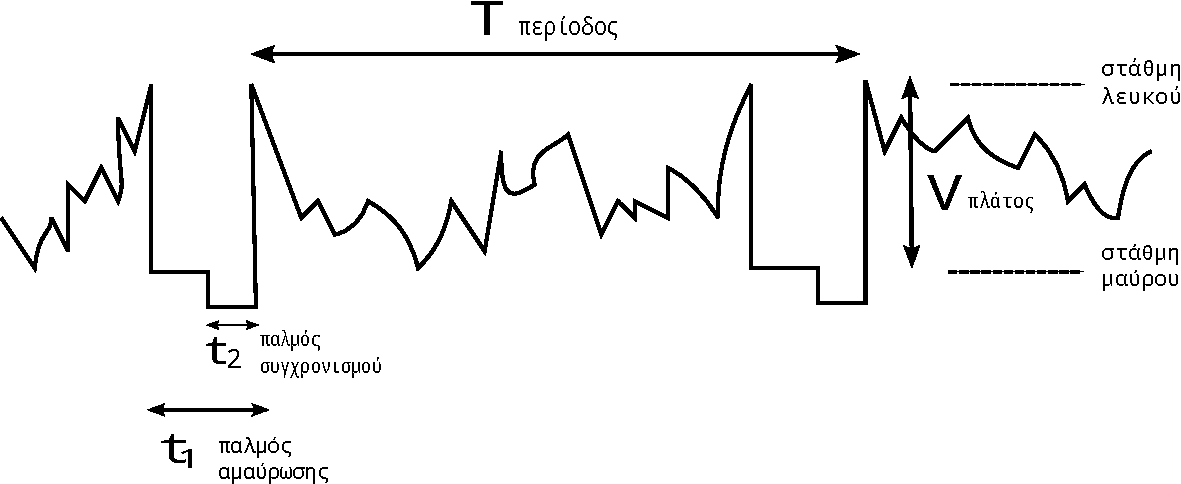
\includegraphics[width=\maxwidth]{signal.pdf}\\[0.3cm]
\caption{Το σήμα εξόδου της κάμερας}
\end{figure}

\newpage
\subsubsection{Laser He-Ne}
Θα χρησιμοποιήσουμε laser Ηλίου-Νέου, που εκπέμπει κόκκινη δέσμη μήκους κύματος $632.8nm$. Η ισχύς εξόδου της δέσμης εμφανίζεται ως συνάρτηση του ρεύματος που διαρρέει το σωλήνα.

\subsubsection{Διαμορφωτής}
Διαμόρφωση της δέσμης ονομάζουμε τον τρόπο με τον οποίο το σήμα της εικόνας υπερτίθεται στη δέσμη του laser. O διαμορφωτής είναι το ηλεκτρονικό κύκλωμα που πραγματοποιεί αυτή τη διαδικασία.

\subsubsection{Απόδιαμορφωτής}
Ο αποδιαμορφωτής στην ουσία κάνει το αντίστροφο πράγμα από το διαμορφωτή. Μετατρέπει το οπτικό σήμα της δέσμης του laser σε ηλεκτρικό. Χρησιμοποιείται μία φωτοδίοδος η οποία έχει την ικανότητα να μετατρέπει την προσπίπτουσα διαμορφωμένη δέσμη σε αντίστοιχες μεταβολές ηλεκτρικού ρεύματος.

\subsubsection{Μόνιτορ}
Είναι μία συσκευή ανάλογη με δέκτη τηλεόρασης. Μετατρέπει το ηλεκτρικό σήμα σε εικόνα.

\section{Εκτέλεση πειράματος}
Στην αρχή συνδέσαμε την κάμερα με το laser και το δέκτη με το μόνιτορ όπως φαίνεται παρακάτω. 

\begin{figure}[h!]
\centering

\includegraphics[width=120mm]{img_1.pdf}\\[0.3cm]
\caption{Πρώτη διάταξη}
\end{figure}

Ευθυγραμμίσαμε τη δέσμη ώστε να πέφτει πάνω στην είσοδο του δέκτη μέχρι να εμφανιστεί η εικόνα στο μόνιτορ. Φέρνοντας το χέρι μας κοντά στην κάμερα, παρατηρήσαμε την ευκρίνεια που είχε η εικόνα στο μόνιτορ καθώς μπορούσαμε να δούμε τους θύλακες της τρίχας.\\\\
Στο επόμενο βήμα, στη θέση της κάμερας βάλαμε τη γεννήτρια και στη θέση του μόνιτορ συνδέσαμε τον παλμογράφο όπως στο σχήμα 3.

\begin{figure}[h!]
\centering
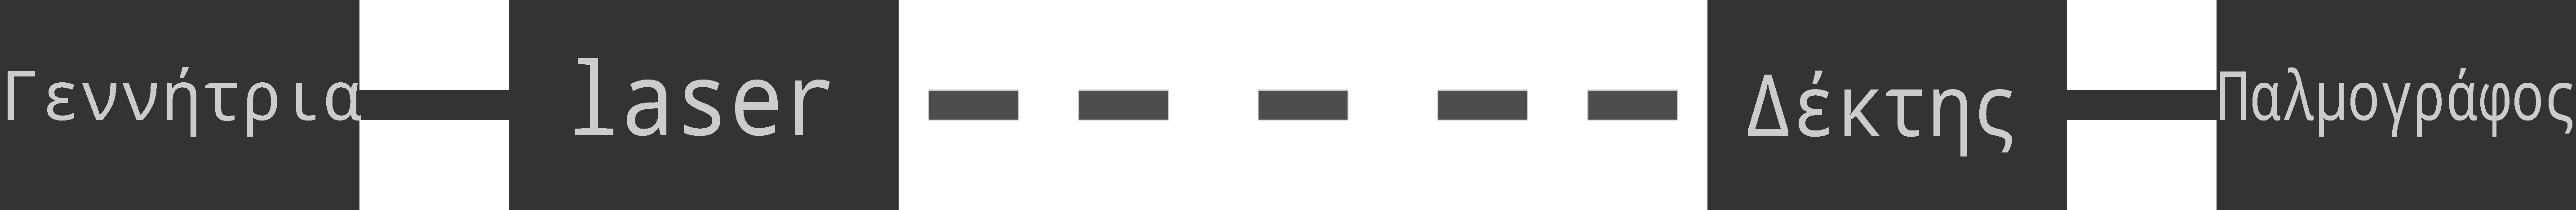
\includegraphics[width=120mm]{img_2.pdf}\\[0.3cm]
\caption{Δεύτερη διάταξη}
\end{figure}

Στη συνέχεια μεταβάλαμε τη συχνότητα από τα 100KHz ως τα 5MHz, στην αρχή με βήμα 100KHz και μετά τα 2MHz με βήμα 1ΜHz. Το σφάλμα ανάγνωσης της γεννήτριας το ορίσαμε $\pm$ 50KHz και του παλμογράφου περίπου $\pm 0.2V$. Τα αποτελέσματα φαίνονται στον πίνακα 1. Η γραφική παράσταση απεικονίζεται παρακάτω. 
Παρατηρούμε πως σε σχέση με τη θεωρητική καμπύλη, το εύρος είναι αρκετά μικρότερο, περίπου 800 KHz.  

\begin{table}[H]
\begin{center}
    \begin{tabular}{ | c | c |}
    \hline
     $f (KHz)$ & $VPP (Volt)$\\ \hline
     100  & 5.0\\ \hline
     200  & 5.0\\ \hline
     300  & 5.0\\ \hline
     400  & 5.0\\ \hline
     500  & 4.8\\ \hline
     600  & 4.6\\ \hline
     700  & 4.2\\ \hline
     800  & 4.0\\ \hline
     900  & 3.8\\ \hline
     1000 & 3.7\\ \hline
     1200 & 3.2\\ \hline
     1400 & 3.0\\ \hline
     1500 & 2.8\\ \hline
     1600 & 2.6\\ \hline
     1700 & 2.4\\ \hline
     1800 & 2.4\\ \hline
     1900 & 2.4\\ \hline
     2000 & 2.2\\ \hline
     3000 & 0.9\\ \hline
     4000 & 0.6\\ \hline
     5000 & 0.4\\ \hline
    \end{tabular}
\end{center}
\caption{Συχνότητα συναρτήσει του πλάτους}
\end{table}

\newpage

Στη συνέχεια συνδέσαμε την κάμερα απ' ευθείας πάνω στον παλμογράφο και καταγράψαμε τα εξής:

\begin{tabular}{l | l}
\hline
$t_{1}=12{\mu}s$ & Παλμός αμαύρωσης\\
$t_{2}=6{\mu}s$  & Παλμός συγχρονισμού\\
$T=64{\mu}s$     & Περίοδος κύματος\\
$V=1Volt$        & Πλάτος κύματος\\
\hline
\end{tabular}

Η κυματομορφή που είδαμε ήταν παρόμοια με την κυματομορφή που είχε και το laser. Μπορούσε κανείς να παρατηρήσει τους παλμούς αμαύρωσης και συγχρονισμού καθώς και τη στάθμη του λευκού και του μαύρου (μέγιστο και ελάχιστο πλάτος αντίστοιχα). Αξίζει να αναφερθεί πως ο παλμός συγχρονισμού ήταν πιο κάτω από τη διαβάθμιση του μαύρου.\\\\
Τέλος, χρησιμοποιήσαμε την προηγούμενη σύνδεση και φέραμε μπροστά στην κάμερα μία εικόνα με παράλληλες άσπρες και μαύρες μπάρες. Αυτό που παρατηρήσαμε στην έξοδο του παλμογράφου ήταν ένας τετραγωνικός παλμός όπως φαίνεται στο Σχήμα 3. Φαίνεται καθαρά η στάθμη του λευκού και του μαύρου.

\begin{figure}[h!]
\centering
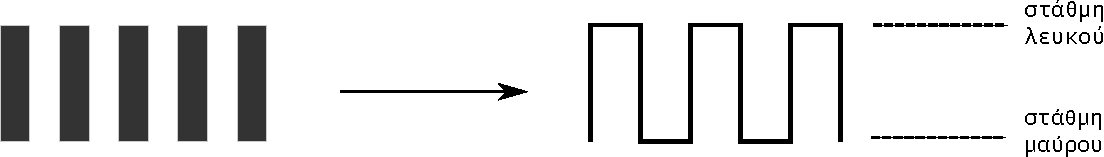
\includegraphics[width=120mm]{bw.pdf}\\[0.3cm]
\caption{Εικόνα τετραγωνικού παλμού}
\end{figure}

\end{document}
